\section{Galois Fields, Polynomial Functions \& Hardware Design}
\label{sec:prelimgf}
%\vspace{-0.035in}

%% We briefly describe the relevant concepts related to Galois fields
%% $\Fkk$; for more details, interested readers may refer to the textbook 
%% \cite{galois_field:mceliece}. 
%% %to put the complexity of the verification problem in perspective, 
%% %to shed some light on the complexity of our design verification, 
%% We also review some VLSI architectures used for Galois field
%% computations \cite{mastro:phd} \cite{acar:1998} \cite{wu:2002}
%% \cite{Knezevic:2008} \cite{eccld} \cite{ecc163}. In our experiments,
%% we have verified custom designs based on these architectures. 

%%%%%%%%%%%%%%%%%%%%%%%%%%%%%%%%%%%%%%%%%%%%%%%%%%%%%%%%%%%%%%%%%%%%%%%%%%%%
%% %\begin{Definition}
%% A finite field, also called a {\bf Galois field}, denoted by $F_q$, is
%% a set of $q$ elements, including two distinguished elements 0 and 1,
%% along with operations $'+'$ and $'\cdot'$ (addition and
%% multiplication) that satisfy the following properties: 
%% \begin{itemize}
%% \item ($F_q, +, 0$) forms an Abelian group.

%% % \begin{itemize}
%% % \item  Closure: $\forall a, b \in F_q, a + b \in F_q$.
%% % \item Associativity: $\forall a, b, c \in F_q, a+(b+c)=(a+b)+c$.
%% % \item Commutativity: $\forall a, b \in F_q, a+b=b+a$.
%% % \item Additive Identity: $\forall a \in F_q, a+0=a$. 
%% % \item Additive Inverse: $\forall a \in F_q$, there is an additive
%% %   inverse element $-a \in F_q$ such that $a+(-a)=0$. 
%% %\end{itemize}

%% \item ($F_q, +, \cdot, 0, 1$) forms a commutative ring with unity.
%% % \begin{itemize}
%% % \item Multiplication closure: $\forall a, b \in F_q, a \cdot b \in
%% %   F_q$.
%% % \item Multiplication Associativity: $\forall a, b, c \in F_q, a \cdot
%% %   (b \cdot c)=(a \cdot b)\cdot c$.  
%% % \item Multiplication Commutativity: $\forall a, b \in F_q, a \cdot b=b \cdot a$. 
%% % \item Multiplication Identity: $\forall a \in F_q, a\cdot 1=a$. 
%% % \item Distributivity: $\forall a, b, c \in F_q, a \cdot (b+c)=(a
%% % \cdot b)+(a \cdot c)$. 
%% % \end{itemize}

%% \item Every non-zero element in $F_q$ has a   multiplicative inverse:
%%   $\forall a \in F_q - \{0\}, \exists a^{-1} \in F_q$ such that $a \cdot
%%   a^{-1}=1$. 

%% \item The number of elements $q$ of the finite field is a
%%   power of a prime integer, i.e. $q = p^k, k \geq 1, p=$ prime. 

%% \end{itemize}
%% %\end{Definition}

A Galois field $\Fq$ is a field with a finite number of elements. The
number of elements $q$ of the field is a power of a prime integer ---
i.e. $q = p^k$, where $p$ is a prime integer, and $k \geq 1$
\cite{galois_field:mceliece}. 
%Galois fields are denoted as ${\mathbb{F}}_{q}$ and also $GF(q
%=p^k)$. 
We are interested in fields where $p = 2$ and $k >1$ --- i.e. {\it
  binary Galois extension   fields} $\mathbb{F}_{2^k}$ --- as they are
widely employed in hardware implementations of cryptography
primitives.  

To construct ${\mathbb{F}}_{2^k}$, we take the polynomial ring
${\mathbb{F}}_2[x]$, where ${\mathbb{F}}_{2} = \{0, 1\}$, and an
irreducible  polynomial $P(x) \in {\mathbb{F}}_2[x]$ of degree $k$, and
construct ${\mathbb{F}}_{2^k}$ as ${\mathbb{F}}_2[x] \pmod{   P(x)}$. As a
result, all field operations are performed 
modulo the irreducible polynomial $P(x)$ and the coefficients are
reduced modulo $p=2$. %=2$; due to which $-1 = +1$ over $\Fkk$. 
Any element $A \in {\mathbb{F}}_{2^k}$ can be represented in polynomial
form as $A = a_0 +  a_1 \alpha + \dots + a_{k-1} \alpha^{k-1}$, where
$a_i \in {\mathbb{F}}_2, i = 0, \dots, k-1$, and $\alpha$ is the root of
the irreducible polynomial, {\it i.e.} $P(\alpha)=0$. 
%The field
%$\Fkk$ can therefore be construed as a $k$-dimensional vector space
%over ${\mathbb{F}}_2$.

%For
%example, $\mathbb{F}_{16} =  \mathbb{F}_2[x] \pmod{ x^4 + x + 1}$. 

%% \debug{
%% The {\it characteristic} of any finite field with
%% unity element $1$ is the least integer $n$ such that $1 + \dots + 1$
%% {\it (n times)} $= 0$. The characteristic of fields of the type
%% ${\mathbb{F}}_{p^k}$ %{\mathbb{F}}_p[x] \pmod{ P(x)}$ 
%% is the prime integer $p$. Since in our
%% case $p = 2$, all fields of the type $\Fkk$, for any given $k$, have 
%% characteristic 2. As a result, all field operations are performed
%% modulo the irreducible polynomial $P(x)$ and the coefficients are
%% reduced modulo $p=2$; due to which $-1 = +1$ over $\Fkk$. 
%% }

%% Any element $A \in \mathbb{F}_{2^k}$ can be represented in polynomial
%% form as $A = a_0 +  a_1 \alpha + \dots + a_{k-1} \alpha^{k-1}$, where
%% $a_i \in \mathbb{F}_2, i = 0, \dots, k-1$, and $\alpha$ is the root of
%% the irreducible polynomial, {\it i.e.} $P(\alpha)=0$. The field
%% $\Fkk$ can therefore be construed as a $k$-dimensional vector space
%% over $\mathbb{F}_2$.



\begin{Example}\label{ex:1}
{\it
Let us construct ${\mathbb{F}}_{2^4}$ as ${\mathbb{F}}_2[x] \pmod{
  P(x)}$, where $P(x)=x^4+x^3+1 \in {\mathbb{F}}_2[x]$ is an
irreducible polynomial of degree $k =4$. Let $\alpha$ be the root of
$P(x)$, i.e. $P(\alpha)=0$.  Any element $A \in {\mathbb{F}}_2[x]
\pmod{ x^4 + x^3 + 1}$ has a representation of the type: $A = a_3 x^3
+ a_2 x^2 +  a_1 x + a_0$ where the coefficients $a_3, \dots, a_0$ are
in ${\mathbb{F}}_2 = \{0, 1\}$. Since there are only 16 such
polynomials, we obtain 16 elements in the field
${\mathbb{F}}_{16}$. Each element in can then be viewed as a 4-bit
vector over ${\mathbb{F}}_2$: ${\mathbb{F}}_{16}=\{(0000),(0001),
\dots (1110),(1111)\}$.  Each element also has an exponential
representation; all three representations are shown in Table
\ref{tab:gfelement}. For example, consider the element $\alpha^{12}$.
Computing $\alpha^{12} \pmod{ \alpha^4+\alpha^3+1} = \alpha + 1
= (0011)$; hence we have the three equivalent representations. 
}

\vspace{-0.1in}
\begin{table}[h]
\begin{center}
{\tiny
\caption{Bit-vector, Exponential and Polynomial representation of
elements in  ${\mathbb{F}}_{2^4} = {\mathbb{F}}_2[x]
\pmod{x^4+x^3+1}$}\label{tab:gfelement}  
\begin{tabular}{|c|c|c||c|c|c|} 
\hline
$a_3a_2a_1a_0$ & Exponential & Polynomial     &$a_3a_2a_1a_0$ & Exponential & Polynomial  \\
\hline
$0000$        & $0$         & $0$            & $1000$ & $\alpha^3$ &  $\alpha^3$\\
\hline
$0001$        & $1$         & $1$            & $1001$ & $\alpha^4$ & $\alpha^3 + 1$\\
\hline
$0010$        & $\alpha$    & $\alpha$       & $1010$ & $\alpha^{10}$&$\alpha^3 + \alpha$  \\
\hline
$0011$        & $\alpha^{12}$& $\alpha + 1$   & $1011$ & $\alpha^5$ & $\alpha^3+\alpha+1$\\
\hline
$0100$        & $\alpha^2$  & $\alpha^2$     &  $1100$ & $\alpha^{14}$ & $\alpha^3 + \alpha^2$\\
\hline
$0101$        & $\alpha^9$   &$\alpha^2 + 1$ & $1101$  &$\alpha^{11}$  & $\alpha^3+\alpha^2+1$\\
\hline
$0110$        & $\alpha^{13}$& $\alpha^2 + \alpha$ & $1110$ & $\alpha^8$& $\alpha^3+\alpha^2+\alpha$\\
\hline
$0111$        &$\alpha^7 $ & $\alpha^2+\alpha+1$ & $1111$ &$\alpha^6$ & $\alpha^3+\alpha^2+\alpha+1$\\
\hline
\end{tabular}
}
\end{center}
\end{table}
\end{Example}




%%%%%%%%%
{\bf Polynomial Functions $f: \Fkk \rightarrow \Fkk$:} 
Arbitrary mappings among $k$-bit vectors can be constructed; each such
mapping generates a function $f: \B^k \rightarrow \B^k$. 
%. Since every
%$k$-bit vector can be construed as an element in $\Fkk$ (as shown in
%the above example), every such function corresponds to a function over
Every such function is also a polynomial function over Galois fields:
$f: \Fkk \rightarrow \Fkk$.  

\begin{Theorem}
From \cite{ff:1997}: 
Any  function $f: \Fq \to \Fq$ is a polynomial function
over $\Fq$, that is there exists a polynomial $\F \in \Fq [x]$ such
  that $f(a) = \F(a)$, for all $a \in \Fq$. 
\end{Theorem}

By analyzing $f$ over each of the $q$ points, one can apply
{\bf Langrange's interpolation formula} and interpolate a polynomial
$\F(x) = \sum_{k=1} ^q  \frac{ \prod_{i \neq k}  (x -x_i)}{\prod_{i \neq k}
  (x_k -x_i)} \cdot f(x_k)$, which is a polynomial of degree at 
most $q-1$ in $x$. One can easily see that $\F(a)=f(a)$ for all $a \in
\Fq$, and $\F(x)$ is therefore the polynomial function representation
of $f$. 

%% \begin{Example} {\it
%% Let $A = \{a_2, a_1, a_0\}$ and $Y = \{y_2, y_1,
%% y_0\}$ be 3-bit vectors.  Consider the function $Y[2:0] = A[2:0]
%% >> 1$, i.e. a {\bf bit-vector right shift} operation on $A$. 
%% The function maps as follows:

%% \begin{center}
%% {\small
%% \begin{tabular}{c|ccc|c||c|ccc|c}
%% $\{a_2a_1a_0\}$  & $A$ &$\rightarrow$& $\{y_2y_1y_0\}$ &$Y$ &
%%   $\{a_2a_1a_0\}$  &$A$&$\rightarrow$& $\{y_2y_1y_0\}$ &$Y$\\
%% \hline
%% 000  &0 &$\rightarrow$& 000 & 0 & 100  &$\alpha^2$ &$\rightarrow$& 010 &  $\alpha$ \\
%% 001  &1 &$\rightarrow$& 000 & 0 & 101  &$\alpha^2 + 1$ &$\rightarrow$&010 & $\alpha$ \\
%% 010  &$\alpha$ & $\rightarrow$ & 001& 1 & 110  &$\alpha^2 + \alpha$&$\rightarrow$& 011 &$\alpha + 1$ \\   
%% 011  &$\alpha + 1$ &$\rightarrow$& 001 &1 & 111& $\alpha^2 + \alpha + 1$ &$\rightarrow$& 011 &$\alpha + 1$\\
%% \hline
%% \end {tabular}
%% }
%% \end{center}

%% If we model this function as $f: {\mathbb{Z}}_{8} \rightarrow
%% {\mathbb{Z}}_{8}$, then using the results of \cite{singmaster}
%% \cite{chen_95} \cite{chen_96}, we deduce that this function is not a
%% polynomial function over ${\mathbb{Z}}_{8}$. However, applying
%% Largange's interpolation formula over ${\mathbb{F}}_{2^3}$, we obtain
%% the following polynomial function representation, $Y =
%% (\alpha^2+1)A^4+(\alpha^2+1)A^2$, where $P(\alpha) = \alpha^3 +
%% \alpha + 1 = 0$. 
%% }
%% \end{Example}

An important property of Galois fields is that for all elements $A \in
{\mathbb{F}}_q, A^q = A$, and hence $A^q - A =  0.$ Therefore, the
polynomial $x^q -x$ {\it vanishes} on all points in
$\Fq$. Consequently, any polynomial $\F(X)$ can be reduced $\pmod{ X^q
  - X}$ to obtain a canonical representation $\F(X) \pmod{X^q - X}$
with degree at most $q-1$. 
%Such {\it vanishing polynomials} will form
%an important part of our formulation.  

\begin{Definition}
Any function $f: \Fq^d \to \Fq$ has a unique canonical representation
(UCR) as polynomial $\F \in \Fq[x_1,\dots, x_d]$ such that all its 
nonzero monomials are of the form $x_1^{i_1}\cdots x_d^{i_d}$ where $0
\leq i_j \leq q-1$, for all $j=1, \ldots d$.
\end{Definition}


\subsection{Hardware Implementations of Galois Field Arithmetic}
% Operations Over $\mathbb{F}_{2^k}$}

{\bf Point Addition over Elliptic Curves:} The main operations of
encryption, decryption and authentication in elliptic curve
cryptography (ECC) rely on {\it point additions} and {\it doubling}
operations on elliptic curves designed over Galois fields. 
%Point multiplication involves a series of addition and doubling of
%points on the elliptic curve. % -- this, in turn, requires finite
%field multiplications.  
%A drawback of traditional approaches is that they require
%point multiplication is that each point addition and doubling 
In general, this requires computation of multiplicative inverses over
the field - which is expensive. Modern approaches represent
the points in projective coordinate systems, {\it e.g.}, the
L$\acute{o}$pez-Dahab (LD) projective coordinate \cite{eccld},
%\cite{ecc:software},
which eliminates the need for multiplicative inverses and improves the
efficiency of these operations. 

%%%

%% \begin{Example}
%% {\it 
%% Consider point addition in L$\acute{o}$pez-Dahab (LD) projective
%% coordinate. Given an elliptic curve: $Y^2 + XYZ = X^3Z + aX^2Z^2 +
%% bZ^4$ over $\mathbb{F}_{2^k}$,   where $X,Y,Z$ are $k$-bit vectors
%% that are elements in $\mathbb{F}_{2^k}$ and similarly, $a, b$ are
%% constants from the field.   Let ($X_3$, $Y_3$, $Z_3$) = ($X_1$, $Y_1$,
%% $Z_1$) + ($X_2$, $Y_2$, $1$)  represent point addition over the
%% elliptic curve.  Then $X_3$, $Y_3$, $Z_3$ can be computed as follows: 

%% \begin{align*}
%% A &= Y_2 \cdot Z_1^2 + Y_1 \\
%% B &= X_2 \cdot Z_1 + X_1 \\
%% C &= Z_1 \cdot B \\
%% D &= B^2 \cdot(C + a Z_1^2) \\
%% Z_3 &= C^2 \\
%% E &= A \cdot C  \\
%% X_3 &= A^2 + D + E  \\
%% F &= X_3 + X_2 \cdot Z_3 \\
%% G &= X_3 + Y_2\cdot Z_3 \\
%% Y_3 &= E\cdot F + Z_3 \cdot G \\
%% \end{align*}
%% }
%% \end{Example}

\begin{Example}
{\it 
Consider point doubling in LD projective coordinate system. Given an
elliptic curve: $Y^2 + XYZ = X^3Z + aX^2Z^2 + bZ^4$.  
Let  ($X_3$, $Y_3$, $Z_3$) = 2($X_1$, $Y_1$, $Z_1$), then $X_3, Y_3,
Z_3$ can be computed as: $X_3 = X_1^4 + b \cdot Z_1^4; ~~Z_3 = X_1^2
\cdot Z_1^2; ~~Y_3 = b Z_1^4 \cdot Z_3 + X_3 \cdot (aZ_3 + Y_1^2 +
bZ_1^4 )$. 
}
\end{Example}

The multiplication and iterative squaring operations in the above
computation are usually implemented using custom-designed Galois field
multipliers, such as the Mastrovito \cite{mastro:1989}, Montgomery
\cite{acar:1998}, Barrett multipliers \cite{Knezevic:2008}, or
composite-field multipliers \cite{cfmulti:1996} --- which are, in
turn, hierarchically designed.  
For example, Montgomery reduction (MR)
computes: $MR(A,B)=A\cdot B \cdot R^{-1} \pmod {P(x)}$, 
where $A,B$ are $k$-bit inputs, $R$ is suitably chosen as
$R={\alpha}^k$, $R^{-1}$ is multiplicative inverse of $R$ in
${\mathbb{F}}_{2^k}$, and $P(x)$ is the irreducible polynomial.
Since Montgomery reduction cannot directly compute $A\cdot B \pmod
{P(x)}$, we need to pre-compute $A\cdot R$ and $B\cdot R$, as shown in
Figure \ref{fig:mm4}.   

\begin{figure}[hbt]
	\begin{center}
	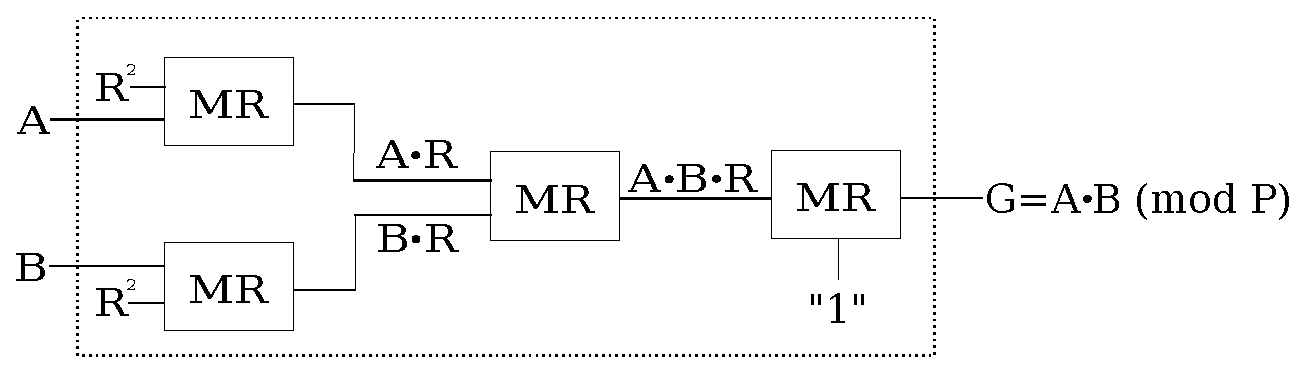
\includegraphics[scale=0.4]{../new_mmcircuit.eps}
	\end{center}
	\caption{{\it Montgomery} multiplication over $\mathbb{F}_{2^k}$
          using four Montgomery reductions.}
	\label{fig:mm4}
\end{figure}

Given a hierarchically designed Montgomery multiplier, we will first
extract polynomials $AR, BR, ABR$ from the sub-circuit blocks. By
analyzing the interconnection of these sub-circuits at word-level, we
can then apply our approach at a higher-level, to extract the function
of the entire circuit. Performing such operations hierarchically, we
will apply our approach to reverse-engineer point-addition circuits
designed using a variety of such Galois field adder and multiplier
circuits.  
